\graphicspath{{fig/model_development/}}

\chapter{Model development}
\label{cha:model_dev}

In this chapter we shall introduce one of the most popular and well studied agent-based
models in the literature: the Vicsek model. The Vicsek model represents a simple alignment
model in which agents interact with neighbours within some given distance. Despite its
simplicity, this model can produce sophisticated dynamics reminiscent of real flocking
events. A phase transition from order to disorder is observed as the amount of noise in
the model is regulated.

The Vicsek model, like many other ABMs, implements a discontinuous interaction rule. With
this, the onset of interaction between individuals is very sensitive to small perturbations
in distances. We consider continuous interaction rules as a biologically-motivated
alternative. Such rules ensure interactions are more robust to small perturbations in
distances, and without the penalty of additional model complexity.

\section{The Vicsek model}

The Vicsek model simulates the movements of $N$ individuals moving with constant speed $v$
(\cref{fig:vicsek_sim}). All movement takes place in a square-cell with periodic boundary
conditions and side length $L$. To initialise a simulation agents are allocated a random
position within the cell, and a random direction of motion. From time $t$ to time $t+1$
agent $i$ updates its position as:
\begin{equation*}
    \bm{x}_{i, t+1} = \bm{x}_{i, t} + \bm{v}_{i, t},
\end{equation*}
where the velocity $\bm{v}_{i,t}$ is constructed to have speed $v$ and direction of motion
$\theta_{i, t+1}$. Updating $\theta_{i,t}$ to $\theta_{i, t+1}$ models how agents update
their directions of motion in light of their neighbours' movements. The ability of
individuals to observe and react to the movements of their neighbours is assumed to be
imperfect, and so a noise term, in the form of a random directional perturbation, is
introduced. In the Vicsek model noise is considered to be uniformly distributed as
$\mathcal{U}(-\eta/2, \eta/2)$. The directional update of agent $i$ can then be expressed
as a realisation from
\begin{equation}
    \label{eq:vicsek_update}
    \theta_{i, t+1} \given \angmean{\theta}_{i, t}, \eta \sim
                   \mathcal{U}(\angmean{\theta}_{i, t} - \eta/2,
                               \angmean{\theta}_{i, t} + \eta/2),
\end{equation}
where $\angmean{\theta}_{i, t}$ represents the average direction of motion of
agent $i$'s neighbours at time $t$.  A weighted circular mean is used to
compute $\angmean{\theta}_{i, t}$ as
\begin{equation}
    \angmean{\theta}_{i, t} = \atantwo\bigg(
        \sum_{j=1}^N \omega_{ij, t} \sin\theta_{j,t},
        \sum_{j=1}^N \omega_{ij, t} \cos\theta_{j,t}
    \bigg).
\end{equation}
With this, the weighting $\omega_{ij, t}$ represents the strength of the interaction
between agent $i$ and agent $j$ at time $t$. In the Vicsek model agent $i$ interacts
with neighbours which are within distance $r$ of its current position. This interaction
can be implemented with the weighting rule
\begin{equation}
    \label{eq:vicsek_interaction}
    \omega_{ij,t} =
    \begin{cases}
        1 & \text{ if } d_{ij, t} \leq r,\\
        0 & \text{ otherwise,}
    \end{cases}
\end{equation}
where $d_{ij,t}$ is the Euclidean-distance between the positions of agent $i$ and agent
$j$ at time $t$:
\begin{equation*}
    d_{ij,t} = \sqrt{(x_{j,t} - x_{i,t})^2 + (y_{j,t} - y_{i,t})^2}.
\end{equation*}

The interaction rule implemented in the Vicsek model represents a discontinuous
interaction, as the interaction kernel is very sensitive to small perturbations in
distances.  More formally, this discontinuity can be shown by considering the value of
$\omega_{ij, t}$ as $d_{ij,t}$ tends to $r$ from above and below.  As $d_{ij,t}$ tends to
$r$ from above it can be seen that $\lim_{d_{ij,t} \rightarrow r^+} \omega_{ij,t} = 0$.
Conversely, as $d_{ij,t}$ tends to $r$ from below we observe: $\lim_{d_{ij,t} \rightarrow
r^-} \omega_{ij,t} = 1$. As the weighting tends to different values as the limit of
$d_{ij,t}=r$ is approached from above and below, we see that there is a discontinuity at
$d_{ij,t}=r$.

The Vicsek model was motivated by models for ferromagnetism. In these models
particles align spin states with neighbouring particles. Although a discontinuous
interaction rule may be appropriate for such models, it is not clear whether the
hard cut-off imposed by the interaction radius is appropriate for biological systems.
Later, we shall introduce models implementing continuous interaction rules as a
biologically-motivated alternative.

Along with the introduction of their model, \cite{vicsek95} examined the polarisation of
simulated flocks as the magnitude of the noise was varied. The polarisation of a flock at
time $t$ was quantified by the absolute value of the normalised velocity of a flock:
\begin{equation}
    v_{a,t} = \frac{1}{Nv} \abs{\,\sum_{i=1}^N \bm{v}_{i,t}\,}.
\end{equation}
At time $t$, a flock moving incohesively, with individual members directed randomly, has
polarisation $v_{a,t}\approx0$. Conversely, a highly polarised flock in which all members
are moving in the same direction at time $t$ has an alignment $v_{a,t}\approx1$. As the
amount of noise in a simulation is increased flocks are observed to transition from an
ordered $v_{a,t}\approx1$ state to a disordered $v_{a,t}\approx0$ state. For a fixed flock
density, smaller flocks are observed to be more resistant to noise than larger flocks.

\begin{figure}[tb]
    \begin{subfigure}[b]{0.5\textwidth}
        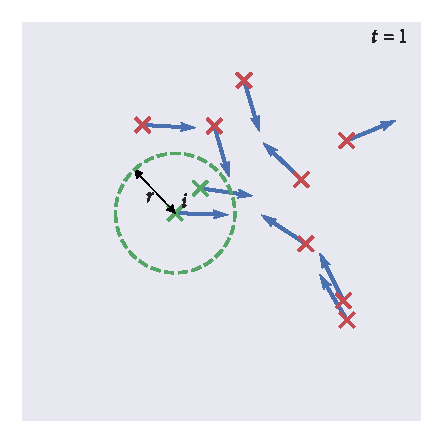
\includegraphics{vicsek_simulation_1.pdf}
    \end{subfigure}%
    \begin{subfigure}[b]{0.5\textwidth}
        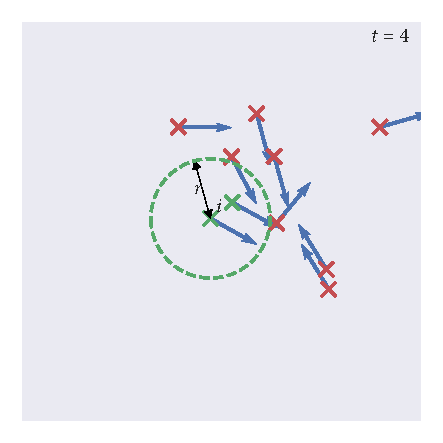
\includegraphics{vicsek_simulation_4.pdf}
    \end{subfigure}
    \begin{subfigure}[b]{0.5\textwidth} 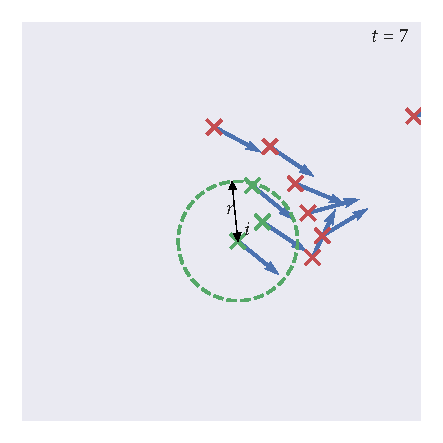
\includegraphics{vicsek_simulation_7.pdf}
    \end{subfigure}%
    \begin{subfigure}[b]{0.5\textwidth}
        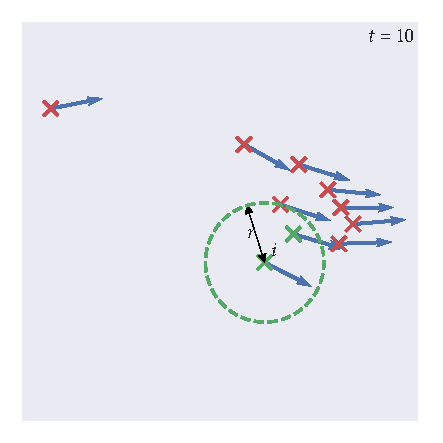
\includegraphics{vicsek_simulation_10.pdf}
    \end{subfigure}
    \caption{Visualisations from a simulation of the Vicsek model. At time $t=1$, $N=10$
        agents are assigned random positions within a square-cell of side length $L=1$.
        Initially, the directions of motion of individuals are realised from a
        $\mathcal{U}(-\pi, \pi)$ distribution. Between time steps agents move with speed
        $v=0.03$, and update directions according to \cref{eq:vicsek_update}, with
        $\eta=\pi/16$. The interaction zone of agent $i$ is illustrated throughout the
        simulation by a circle of radius $r$ centred at $\bm{x}_{i,t}$. The positions of
        neighbours within agent $i$'s interaction zone are visualised with a green cross.
        Individuals which lie outside of agent $i$'s interaction zone have their positions
        denoted by a red cross.}
        \label{fig:vicsek_sim}
\end{figure}

\subsection{Considerations of stochasticity}

Inspired by models of interacting particles, the uniformly distributed noise implemented in
simulations of the Vicsek model is analogous to temperature in a physical system. However,
it is not clear whether this distribution is a reasonable choice for biologically-motivated
systems. In much of the literature authors instead assume that noise is normally
distributed. In this case an agent's directional update typically takes the form:
\begin{equation*}
    \theta_{i,t+1} \given \angmean{\theta}_{i,t}, \sigma_Y \sim
        \mathcal{N}(\angmean{\theta}_{i,t}, \sigma_Y).
\end{equation*}

Throughout this work we shall also consider the possibility that the noise experienced by
individuals is distributed according to some generalised Student's $t$-distribution with
$\nu$ degrees of freedom. In this situation, the directional update of agent $i$ is given
as:
\begin{equation*}
    \theta_{i,t+1} \given \angmean{\theta}_{i,t}, \nu, \sigma_Y \sim
    t_{\nu}(\angmean{\theta}_{i,t}, \sigma_Y).
\end{equation*}
The Student's $t$-distribution allows more weight in its tails than the normal
distribution permits. However, as $\nu\rightarrow\infty$ the Student's $t$-distribution
with location $\mu$ and scale $\sigma_Y$ converges to a normal distribution with mean and
standard deviation corresponding to these location and scale parameters.  Although the
Student's $t$-distribution represents a more flexible noise structure, it also comes at
the cost of model complexity: with the introduction of the degrees of freedom as an
additional model parameter.

\subsection{Boundary conditions \& trajectory plots}

Recall that all simulations of the Vicsek model take place in a square-cell with periodic
boundary conditions and side-length $L$. In this way the density of a cell remains
constant throughout a simulation. However, implementing periodic boundary conditions when
we attempt to mimic real flocking events is clearly inappropriate. Instead, we shall
consider simulations to take place in the unrestricted continuous domain represented by
$\mathbb{R}^2$.  On top of realism, performing simulations in this unrestricted domain
allows more informative visualisations of the resulting data, as in
\cref{fig:example_traj}. Here we are able to visualise the positions of agents throughout
a simulation in a single graphic.

\begin{figure}[tb]
    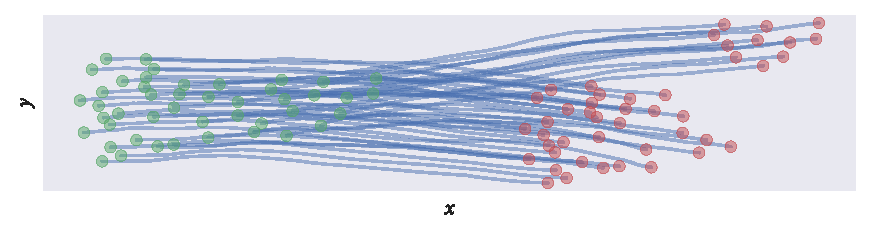
\includegraphics{example_traj_plot.pdf}
    \caption{A trajectory plot representing the movements of $N=45$ agents moving through
        the unrestricted continuous domain $\mathbb{R}^2$. Agents are initially positioned
        at the locations represented by the green markers. The model is simulated for
        $200$ time steps. The red markers represent the positions of agents at the end of
        a simulation. Blue lines represent the trajectories of motion of individual agents
        throughout the simulation.}
    \label{fig:example_traj}
\end{figure}

\section{Continuous interaction models}

It has been seen that the interaction rule implemented in the Vicsek model exhibits a
discontinuity. This discontinuity represents two concerns for the authors. Firstly, the
biological realism of an interaction rule implementing a hard cut-off is brought into
question. Secondly, the ability to fit such a model to data is seen to be potentially
problematic: effectively exploring the sample space of a discontinuous target
distribution can be difficult.

Such concerns can be addressed by considering variations of the Vicsek model in which
continuous interaction rules are implemented. The authors consider that such rules
represent more biologically realistic behaviours. In addition to this, the MCMC algorithms
used to draw samples from our posterior beliefs are expected to be better behaved for the
models implementing continuous interaction rules.

\subsection{Metric models}

Metric models, of which Vicsek is an example, implement weighting rules which are
explicitly distance-dependant. Here we shall motivate two novel metric interaction rules.
We propose that the weighting rules introduced represent intuitive and biologically
realistic rules. \cref{fig:weighting_rules} visualises the interaction rule of Vicsek,
along with the two novel interaction rules to be introduced.

\begin{figure}[tb]
    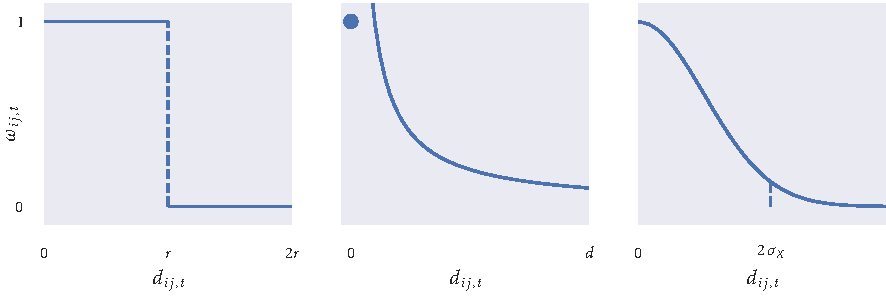
\includegraphics{weighting_rules.pdf}
    \caption{Visualising the relationship between interaction strength $\omega_{ij,t}$ and
        distance $d_{ij,t}$ for three different weighting rules. From left to right we
        visualise: the Vicsek interaction (\cref{eq:vicsek_interaction}), the power-law
        weighted interaction (\cref{eq:power_law_interaction}), and the Gaussian weighted
    interaction (\cref{eq:gaussian_interaction}).}
    \label{fig:weighting_rules}
\end{figure}

\subsubsection{Power-law interaction}

A power-law relationship between two quantities is realised when a relative change in
one quantity results in a proportional change in the other quantity. Power-law
relationships are found frequently in physical and biological systems, and so represent a
natural choice of interaction rule to investigate.

For the power-law weighted model we assume that the interaction strength between
individuals decays as some power-law relationship with their distance apart:
\begin{equation}
    \label{eq:power_law_interaction}
	\omega_{ij,t} =
	\begin{cases}
		1                  & \, \text{if } d_{ij,t} = 0, \\
		d_{ij,t}^{-\alpha} & \, \text{otherwise}.
	\end{cases}
\end{equation}
The interaction of the Vicsek model is parameterised by the radius $r \geq 0$. Here the
interaction is parameterised by some $\alpha\in\mathbb{R}^+$. The parameter $\alpha$
controls the rate at which the interaction strength between individuals decays. 

In this model, the closer a neighbour to agent $i$, the more influence it has over agent
$i$'s behaviour. Conversely then, the further away a neighbour is from the position of
agent $i$, the less influence it has on agent $i$'s movements. The rate at which influence
decays is controlled by the value of $\alpha$. Small values of $\alpha$ represent a more
gradual decay of influence with distance, whereas large values of $\alpha$ correspond to a
weighting which decays more rapidly.

This interaction rule, although continuous for $d_{ij,t} > 0$, exhibits a discontinuity at
$d_{ij,t}=0$. Although this may present a problem theoretically, in practice we do not
consider that this should pose an issue.

\subsubsection{Gaussian interaction}

Similar to the power-law weighted model, in the Gaussian weighted model the influence
which neighbour $j$ exerts over agent $i$ is inversely proportional to their distance
apart; the further away a neighbour the less influence it exerts. The Gaussian weighted
interaction is continuous over all $d_{ij,t}$, and can be expressed as:
\begin{equation}
    \label{eq:gaussian_interaction}
	\omega_{ij,t} =
	\frac{1}{\sqrt{2\pi\sigma_X^2}}
	e^{-\frac{1}{2}\big(\frac{d_{ij,t}}{\sigma_X}\big)^2}.
\end{equation}

From \cref{eq:gaussian_interaction} the parameter $\sigma_X$ can be seen to control the
length scale over which interaction takes place. Small values of $\sigma_X$ detail a
weighting function which is very peaked around agent $i$'s position. As $\sigma_X
\rightarrow \infty$ the weighting approaches a schema in which all neighbours in the flock
are awarded the same weight. This limiting behaviour is equivalent to that of Vicsek as
$r\rightarrow\infty$, and the power-law weighted model as $\alpha\rightarrow0$.

Although the Gaussian model implements a similar interaction kernel to that of the
power-law weighted model, there remains differences in their functional forms.  Most
notably is that the power-law interaction represents a convex weighting function, whereas
the Gaussian interaction is a concave weighting (\cref{fig:weighting_rules}). The Gaussian
model also has some inherent length scale, expressed by the parameter $\sigma_X$, whereas
the power-law weighted interaction is scale-free.

\subsection{Topological models}

Much interest in topological interaction rules was recently generated by
\cite{ballerini08}. Topological rules represent a different type of interaction to metric
rules. Here, agents interact with their $k\in\mathbb{N}$ nearest neighbours, regardless of
their distance apart. This interaction rule was motivated by simulations which suggested
that flocks implementing topological rules were more resistant to perturbations, such as
those by predators, than those implementing metric rules. As such, it was argued that
topological interaction rules offer an evolutionary advantage to flocks over metric
interaction rules.
It was also posed that the cognitive limits of individuals puts some upper bound on the
number of neighbours which agents can interact with at any one time.

Whilst retaining the form of the topological rule, we look to relax the constraint that
agents may only interact with some \emph{integer} number of closest neighbours.  Instead,
we allow an agent to interact with some $k\in\mathbb{R}^+$ nearest neighbours.  This
allows partial neighbours, which may make some lesser contribution to an agent's behaviour.

For some $k\in\mathbb{R}^+$ we say that each agent gives weighting $1$ to its $\floor{k}$
nearest neighbours, weighting $k - \floor{k}$ to its $\ceil{k}$-th nearest neighbour, and
weighting $0$ to all other agents, where $\floor{\cdot}$ and $\ceil{\cdot}$ are the floor
and ceiling function respectively. More concisely, we can express this as the weighting
\begin{equation}
	\omega_{ij,t} =
	\begin{cases}
		1           & \, \text{if } d_{ij, t} \leq \min_j(d_{ij,t},\, \floor{k}), \\
		k-\floor{k} & \, \text{if } d_{ij, t} = \min_j(d_{ij,t},\, \ceil{k}),     \\
		0           & \, \text{otherwise,}
	\end{cases}
\end{equation}
where $\min_j(d_{ij,t},\, k)$ is the distance to agent $i$'s $k$-th closest neighbour at
time $t$. 

\section{Behavioural \& biological variation}

In all the model variations considered thus far, there has been no allowance for
behavioural or biological variation within flocks. That is, presented with the same
circumstances, all of our agents would behave identically. This is despite our
understanding of the importance of biological variation in nature.

Within a single flock, we may reasonably expect there to be variation in the age,
cognitive ability, social standing and physical attributes of the individuals. Naturally
then, it seems reasonable to suggest that as the attributes of individuals may vary, then
the behavioural response of individuals to a particular set of circumstances may vary too.
This is in keeping with the observation that the orientation abilities of migrating
raptors is age dependent \parencite{thorup03}.

This isn't to say that models allowing intra-flock variation haven't been considered
before. Particularly memorable was the work of \textcite{couzin05}, which simulated flocks
of individuals partitioned into a group of leaders and a group of followers. The two groups
interacted according to different behavioural rules. Followers sought only to amend their
directions in response to the movements of their neighbours. Whereas leaders balanced
their desire to interact with neighbours and their desire to move in a particular
direction (for example, toward a migratory of foraging goal).

Instead of dividing agents into distinct behavioural categories, we permit a range of
behavioural responses by allowing interaction and noise parameters to vary between
individuals. Some agents may be more or less susceptible to noise than others. Consider
then that agent $i$ experiences noise distributed according to a generalised Students
$t$-distribution with $\nu$ degrees of freedom and scale $\sigma_{Y_i}$. Agent $i$'s
directional update is then given as
\begin{equation*}
    \theta_{i,t+1} \given \angmean{\theta}_{i,t}, \nu, \sigma_{Y_i} \sim
    t_{\nu}(\angmean{\theta}_{i,t}, \sigma_{Y_i}).
\end{equation*}

In addition to allowing noise parameters to vary within a flock, we also seek to allow
interaction parameters to vary within a flock. In the case of Vicsek, agent $i$ would then
interact with neighbours positioned within distance $r_i$. This corresponds to the
weighting rule:
\begin{equation}
    \label{eq:vicsek_interaction}
    \omega_{ij,t} =
    \begin{cases}
        1 & \text{ if } d_{ij, t} \leq r_i,\\
        0 & \text{ otherwise.}
    \end{cases}
\end{equation}
A similar allowance can be made for the power-law weighted, Gaussian weighted and
topological models considered.

\subsection{Imposing hierarchy}

Rather than considering the individual interaction and noise parameters as completely
independent, we can consider them as being realisations from a population-level
distribution. Hierarchical models allow us to incorporate this extra level of structure
into our models.

Hyperparameters are introduced as parameters of the specified population-level distribution.
Hyperpriors are then specified to reflect the practitioners beliefs about feasible values
of the hyperparameters.

The noise and interaction parameters in our models are all strictly positive, and not
bounded above. As such, we shall assume that the population distributions for these
parameters follow some gamma distribution. Consider, for example, that the noise
parameters $\sigma_{Y_i}$ are distributed according to some gamma distribution with shape
$\alpha_Y$ and rate $\beta_Y$. More concisely, we consider our noise parameters as being
distributed according to
\begin{equation}
    \label{eq:noise_hier}
    \sigma_{Y_i} \sim \Ga(\alpha_Y, \beta_Y).
\end{equation}
As such, our hyperparameters here are $\alpha_Y$ and $\beta_Y$. The practitioner is then
required to specify hyperpriors: their prior beliefs about plausible values for $\alpha_Y$
and $\beta_Y$. It can be hard to get an intuitive feel for plausible values for the shape
and rate parameters, and so we shall instead re-parameterise our population-level
distribution in terms of the mean and variance. Consider that the mean and variance of the
gamma distribution can be computed as $m_Y = \alpha_Y / \beta_Y$ and $v_Y =
\alpha_Y/\beta_Y^2$ respectively. From these two relations it can be seen that $\alpha_Y =
m_Y^2 / v_Y$ and $\beta_Y = m_Y / v_Y$. \cref{eq:noise_hier} can then be re-expressed as:
\begin{equation}
    \sigma_{Y_i} \sim \Ga\bigg(\frac{m_Y^2}{v_Y}, \frac{m_Y}{v_Y}\bigg).
\end{equation}












